%!TEX TS-program = xelatex
%!TEX root = ../../maxwell2018thesis.tex

\chapter[A Background of Stopping in IIR]{Stopping in Interactive\\Information Retrieval}\label{chap:stopping_background}
Towards the end of Chapter~\ref{chap:ir_background}, we examined a number of different evaluation measures typically employed in~\gls{acr:ir} and~\gls{acr:iir} studies. In particular, we emphasised the notion of different \emph{stopping models} that are implicitly encoded within these measures, ranging from the na\"{i}ve to more representative approaches of a real-world searcher's \emph{stopping behaviours.}

\begin{figure}[h]
    \centering
    \vspace{4mm}
    \resizebox{1\hsize}{!}{
    
\includegraphics{figures/ch3-stopsign.pdf}}
    \label{fig:stopsign}
    \vspace{-5mm}
\end{figure}

In this chapter, we provide an overview of work undertaken in the field of~\gls{acr:iir} that explicitly examine the stopping behaviours of searchers. We enumerate on a number of different \emph{stopping heuristics} that attempt to quantify when searchers should stop examining results, before examining \emph{theoretical frameworks} that provide insight and explanation into why and when searchers stop. We then examine a number of different \emph{user studies} that have examined stopping behaviours. Before examining these prior works, we first consider why examining the stopping behaviour of searchers is important to the field, and to the future development of the retrieval systems and their interfaces that we use extensively today.

\section{Why Stopping?}\label{sec:stopping_background:why}
Knowing when to stop is a fundamental aspect of human thinking and behaviour. Humans and other animals, when interacting with the world, will employ some form of \emph{stopping criterion} (or criteria) to decide when they should stop~\citep{nickles1995judgment}. As an example, a shopper who is looking to purchase a new smartphone will stop shopping around once he or she has obtained sufficient information on which new smartphone to purchase. Once their case notes for a patient have been compiled, a medical doctor will then be in a position to diagnose the patient's ailment. In the context of search, numerous reasons exist why searchers stop. Perhaps searchers stop because they have satisfied their information need, have become frustrated with the lack of potentially relevant information -- or because of some external factor, such as a time constraint that has been imposed upon them.

The decision of when to stop is not exclusively due to such external factors to the decision maker, but rather from a series of \emph{internal, cognitive factors} of their thinking process~\citep{nickles1995judgment}. For example, an individual who is hungry will stop eating once he or she feels full, rather than stopping when all of the food presented to them has been consumed. Empirical research has over the years demonstrated that individuals, regardless of the task presented to them, will frequently stop prematurely. Indeed, this na\"{i}ve behaviour demonstrates that individuals may be willing to go with what \emph{``sounds right''} to them -- often minimising the cognitive effort that is required at the expense of greater accuracy~\citep{perkins1983difficulties}. However, when searching, this lower level of potential accuracy does lead to individuals making a greater number of errors in their decision making~\citep{baron1988heuristics}. Searchers overlook important elements, and potentially miss out useful information~\citep{fischhoff1977cost_benefit, fischhoff1978fault, shafir1992thinking}, with the individual then failing to consider alternatives~\citep{farquhar1993decision_structuring}.

Based upon prior research into stopping behaviours, it is clear that such a decision is driven primarily from internal factors. As such, we then consider: \emph{what aspects of the decision maker's thinking processes prompt him or her to stop assessing the information provided?} Knowing when to stop requires that the individual in question makes a \emph{judgement} regarding the sufficiency of the information obtained, and whether or not additional information is required~\citep{browne2004stopping_rules}. This judgement is normally characterised by both the completeness and correctness of the information obtained thus far~\citep{smith1991belief}. These claims can be mirrored by qualitative studies on examining stopping behaviour. Here, researchers have found that searchers stop examining search results simply because what they have found previously is \emph{``good enough''}~\citep{zach2005enough_is_enough} to satisfy their underlying information need. This finding echoes the reasoning that individuals would be happy to stop when what they have found \emph{``sounds right''}~\citep{perkins1983difficulties}.

\begin{figure}[t!]
    \centering
    \resizebox{1\hsize}{!}{
    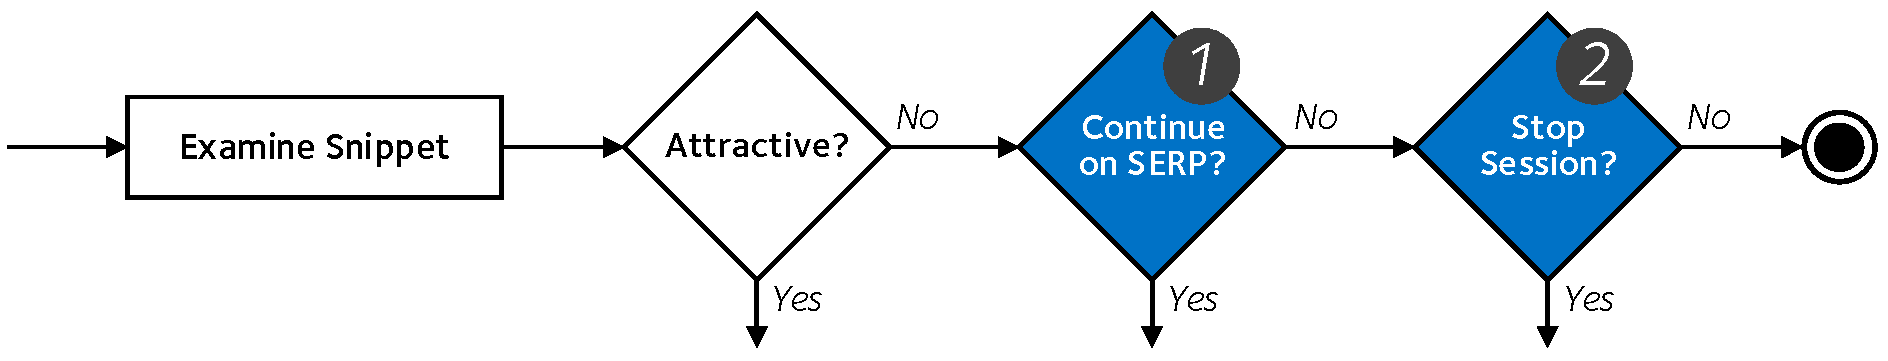
\includegraphics{figures/ch3-two_points.pdf}}
    \caption[Two established \emph{stopping decision points}]{Excerpts from various searcher models, highlighting two established \emph{stopping decision points.} These are modelled as points at which searchers can stop performing a given action. These are illustrated as blue diamonds. The two points consider \blueboxbold{1} \emph{\gls{glos:summary_stopping}} (often called \emph{snippet level} or \emph{query level stopping}), and \blueboxbold{2} \emph{\gls{glos:session_stopping}}.}
    \label{fig:model_two_points}
\end{figure}

\subsection{Stopping Decision Points}\label{sec:stopping_background:why:points}
In Section~\ref{sec:ir_background:user:models}, we discussed a number of searcher models that are considered to be an improvement over the traditional~\gls{acr:trec}-style searcher model, a model that is agnostic of a searcher's interactions. The more advanced models considered two distinct \emph{stopping decision points} that capture specific points during the interaction process where a searcher can stop their current activity, and move onto the next step in the process. These stopping decision points are illustrated in an excerpt of a typical searcher model flowchart, as shown in Figure~\ref{fig:model_two_points}. Both established stopping decision points are discussed below.

\begin{itemize}
    \item[\blueboxbold{1}]{\darkblueboxbold{Result Summary Level Stopping} Traditionally called \emph{snippet level stopping} or \emph{query level stopping} in the literature\footnote{The phrase \emph{\gls{glos:summary_stopping}} is used in this thesis to avoid confusion with a new~\gls{glos:serp_stopping} decision point, discussed in depth in Section~\ref{sec:csm:advancements:stopping} on page~\pageref{sec:csm:advancements:stopping}.}, this stopping decision point considers the depth at which a searcher will stop examining a list of ranked results. After stopping at this point, the searcher can continue the search session by issuing a further query.}
    \item[\blueboxbold{2}]{\darkblueboxbold{Session Level Stopping} This second stopping decision point considers the point at which a searcher will stop their search session in its entirety. As such, this stopping decision point is regarded as terminal to the search session.}
\end{itemize}

In particular,~\gls{glos:session_stopping} is considered when a searcher must decide, for example, if they have met their overall search goal, have run out of time or queries, or simply have become so frustrated with a lack of relevant content that they would rather abandon their search. These stopping decision points can be operationalised in a variety of different ways, as we explore in the remainder of this chapter. Chapter~\ref{chap:csm} also proposes an additional, third stopping decision point that we will consider in a later contributory chapter of this thesis.

\section{Stopping Heuristics}\label{sec:stopping_background:heuristics}
Considering the above, researchers have over several decades devised a number of different high level \emph{stopping rules} -- hereafter referred to as \blueboxbold{stopping heuristics} -- as a means of encoding a searcher's aforementioned sense of what is \emph{``good enough''}~\citep{zach2005enough_is_enough} -- or even what can be considered as \emph{not good enough}.

Stopping heuristics have been investigated in \emph{decision-making} research. A number of normative stopping heuristics have been identified. As examples,~\cite{busemeyer1988deferred_decision_making} considered the expected loss from terminating information acquisition.~\cite{kogut1990sunk_costs} examined the expected value of additional information. Other examples of normative stopping heuristics are demonstrated by~\cite{pitz1969information_seeking} and~\cite{busemeyer1988deferred_decision_making}.

However, as outlined by~\cite{browne2004stopping_rules}, these heuristics usually fail to describe the actual cognitive behaviours of the decision makers. Such heuristics often assume that the decision maker must \emph{think ahead} to the final decision of when to stop, enabling them to assess the value of additional information~\citep{busemeyer1988deferred_decision_making}. This is an inherently difficult task for decision makers to undertake, due to the limited working memory capacity of a human. We are simply unable to cognitively process all of the information attained to make a decision considering all possible outcomes~\citep{browne2004stopping_rules}.~\cite{nickles1995judgment} agreed, stating that normative stopping heuristics made implicit assumptions about the mental activities of the decision maker, especially in terms of mental scaling and weighting. No clear cognitive perspective has yet been provided to address the cognitive mechanisms and/or assumptions of the decision maker's thinking.

\cite{nickles1995judgment} identified two distinct approaches to considering the cognitive processes involved in decision making: \blueboxbold{judgement}, where an individual assesses a context to choose a course of action; and \blueboxbold{reasoning}, where an individual convinces himself or herself that a particular understanding of the scenario is correct. Research in this area of decision making typically assumed that when assessing a particular scenario (or presented information), a decision maker would draw upon the available evidence and use their judgement to make a decision as to how to proceed~\citep{reisberg1997cognition}. This assumption was implicitly used in the normative stopping heuristics outlined above. An alternative way to consider what a decision maker undertakes revolves around the notion that taking a decision is dominated by his or her ability to reason. Drawing on the available evidence, \emph{arguments} can be constructed to reach an overall conclusion. This is known as \emph{belief assessment}~\citep{benson1995belief_assessment}, where the individual determines their degree of belief in the conclusion that has been reached.

With the inherent limitations of the normative stopping rules in mind -- and the two categorisations defined above, we now enumerate a number of different stopping heuristics that are better able to represent a searcher's cognitive processes, considered as either \emph{judgement-based} or \emph{reasoning-based.} We enumerate these heuristics below in their two classifications.

% With these inherent limitations in mind, seminal work in this area was undertaken by~\cite{nickles1995judgment} who provided a broad classification for different explicitly defined stopping heuristics in the literature. These heuristics consider a searcher's cognitive processes and are considered as either \emph{judgement-based heuristics} and \emph{reasoning-based heuristics.} The heuristics we consider are enumerated below, split across the two aforementioned classifications.
%
% typically, decision makers when drawing upon evidence uses their judgement to work out whether something is good or not. and judgement is the evaluation of the evidence to make a decision. (Reisberg, D, 1997)
%
% now in contrast to this, nickles states that assessment onsiders an individual's attempt to form some belief about the event of interest (i.e. finding information). and that this is dominated by the individual's ability to reason about what has been found. drawing on the available evidence and using reasoning, the individual constructs arguments to reach a conclusion~\citep{benson1995belief_assessment}.




% Cognition: Exploring the science of the mind. Reisberg, D


\begin{itemize}
    \item{\darkblueboxbold{Judgement-based Heuristics} These heuristics are defined as when a decision maker maintains some mental threshold along a key dimension and a running total of the number of occurrences of this measure. More details are provided in Section~\ref{sec:stopping_background:heuristics:judgement}.}
    \begin{itemize}
        \item{\blueboxbold{Satisfaction and Frustration} These heuristics consider a decision maker's satisfaction with what they have found during the course of their search \emph{(satisfaction} or \emph{satiation),} or their tolerance to non-relevance \emph{(frustration} or \emph{disgust).}}
        \item{\blueboxbold{Difference Criterion} This heuristic concerns the notion of whether a decision maker is learning anything new by examining more documents.}
        \item{\blueboxbold{Magnitude Threshold} This heuristic concerns a decision maker's belief that the information that they have found provides sufficient evidence to prompt him or her to stop searching for further information.}
        \item{\blueboxbold{Single Criterion} A \emph{single criterion} to the decision maker's information need is considered in this stopping heuristic.}
    \end{itemize}
    
    \item{\darkblueboxbold{Reasoning-based Heuristics} This classification concerns the \emph{mental representation} of the given topic for which a searcher is seeking information. In other words, the mental representation is formed from a series of (perhaps contrasting) points. When combined together, a decision can be made as to the suitability of the information found.}
    \begin{itemize}
        \item{\blueboxbold{Representational Stability} This stopping heuristic concerns the notion of the decision maker's mental model of the topic and the \emph{stabilisation point.}}
        \item{\blueboxbold{Propositional Stability} Here, a series of potential conclusions regarding the underlying information need are formed, with these arguments needing to be satisfied to feel sufficiently satisfied to stop.}
        \item{\blueboxbold{The Mental List} A mental list of aspects is constructed, with each item on the list needing to be addressed by the decision maker before stopping occurs.}
    \end{itemize}
\end{itemize}

These were devised largely as ways of modelling the~\glsfirst{acr:esl}~\citep{cooper1968expected_search_length}, as briefly discussed in Section~\ref{sec:ir_background:evaluation:system:esl}.~\cite{nickles1995judgment} also proposed a number of stopping heuristics that are discussed in subsequent sections, with discussion expanded to include additional heuristics defined by other researchers. We now address each of the two classifications, explaining each of the different heuristics enumerated above in detail.

\subsection{Judgement-Based Heuristics}\label{sec:stopping_background:heuristics:judgement}
As discussed previously, a judgement-based stopping heuristic is defined as when a decision maker is assumed to set and consistently maintain a mental threshold along some form of key dimension (e.g. determining the seemingly relevant from non-relevant), and to keep a running total of the measure relative to the dimension in question~\citep{gettys1979hypothesis, nickles1995judgment}. When the measure meets or exceeds this set threshold, the searcher will then stop searching for information. Each of the judgement-based heuristics we consider in this thesis are discussed in turn below.

\subsubsection{Satisfaction and Frustration}\label{sec:stopping_background:heuristics:frustration}
Two of the earliest stopping heuristics defined in the literature are by~\cite{cooper1973retrieval_effectiveness_ii}, who consider a searcher's tolerance encountering non-relevant material, and how satisfied they become when encountering relevant material. The heuristics were originally defined as a means for estimating the utility a searcher can attain when interacting with a retrieval system. While the means of which~\cite{cooper1973retrieval_effectiveness_ii} estimated the utility of search are not of key relevance to this thesis, the work on stopping heuristics is. The \emph{satisfaction point} and \emph{frustration point} stopping heuristics are considered to be judgement-based heuristics, as they rely solely on the searcher's notion of what constitutes a relevant document. Both consider counts of the number of (non-)relevant documents observed.

\blueboxheader{Satisfaction Point}
The \emph{satisfaction point} heuristic considers the point at which a searcher has found enough material to consider his or her search a success. This is achieved by considering the amount of material found that has been judged to be relevant. It can easily be imagined that such a heuristic would apply directly to both result summary level stopping (i.e. \emph{find $x$ relevant documents on this~\gls{acr:serp}}) and session level stopping (i.e. \emph{find $x$ relevant documents}). This heuristic is also called the \emph{satiation heuristic}~\citep{simon1955satiation} (see below). This heuristic can be considered as a decision making process...

\begin{quote}
    \emph{``[...]through which an individual decides when an alternative approach or solution is sufficient to meet the individuals' desired goals rather than a perfect approach.''}
    \attrib{\cite{simon1971decision}}
\end{quote}

This suggests that a searcher employing the satisfaction stopping heuristic would stop searching as soon as certain conditions arise, instead of after they have exhaustively considered all available information~\citep{march1994primer}. Conditions could include acceptance of the results; discomfort; boredom; time limits; and the \emph{snowballing} of information~\citep{mansourian2007search}, where the repetition or saturation of information occurs.

\blueboxheader{Frustration Point}
In a converse fashion to the satisfaction point heuristic, the \emph{frustration point} heuristic considers a searcher's overall \emph{tolerance to non-relevance} by stopping after being sufficiently frustrated by the results presented to the searcher. This heuristic is also called the \emph{disgust heuristic} in the literature (see below).

The two relatively straightforward heuristics defined above makes a searcher's interactions with a ranked list of results \emph{inherently adaptive.} In other words, given a set of results, his or her behaviour will change with respect to the perceived quality of the ranked list. As a reminder, this would not necessarily mean considering the system's effectiveness measures, but rather user-focused measures such as interactive precision and recall, as discussed previously in Section~\ref{sec:ir_background:evaluation:user:ipr}.

\blueboxheader{Combining Satisfaction and Frustration}
Perhaps due to the relative simplicity of the two aforementioned heuristics, identical approaches have been defined elsewhere in the literature.~\cite{kraft1979stopping_rules} later defined three further stopping heuristics, two of which are the \emph{satiation} (as per~\cite{simon1955satiation}) and \emph{disgust} heuristics. In essence, the rules defined by~\cite{kraft1979stopping_rules} are the same satisfaction and frustration heuristics as previously defined by~\cite{cooper1973retrieval_effectiveness_ii}. Within the satiation rule, a searcher will stop after becoming \emph{satiated} by finding a number of documents considered to be relevant, while the disgust rule considers a searcher's disgust at finding a number of non-relevant documents.

\cite{kraft1979stopping_rules} also proposed a third heuristic that combines both satisfaction/satiation and frustration/disgust together into a single heuristic. Here, a searcher following such an approach would be inclined to stop examining content if they were either satisfied with what had been found, or frustrated by having to trawl through material judged to be non-relevant (thus considering multiple criteria). The stopping point would be whatever of the two conditions are met first. Indeed,~\cite{kraft1979stopping_rules} demonstrated that the~\gls{acr:esl} of a searcher could be approximated using each of the two stopping heuristics by considering the size of the retrieval set, the number of relevant documents a searcher wished to obtain, and the number of non-relevant documents a searcher would be willing to tolerate. The number of documents required to consider a search as successful is dependent upon whether the search task is high precision (where one would stop comparatively early), or high recall (where one would stop comparatively later), as hypothesised by~\cite{bates1984thirty_items}.

\subsubsection{Difference Threshold}\label{sec:stopping_background:heuristics:difference}
The \emph{difference threshold heuristic}~\citep{nickles1995judgment} concerns whether a new document is providing a searcher with additional, useful content about their information need. Here, the searcher is assumed to keep an internal record of the information that has been consumed along some key dimension. The searcher is also assumed to use this internal record of what has been assessed to compare a new document with previously examined content. When the difference between the new and existing information falls below some internal difference threshold, the searcher stops as nothing new is being learnt.

\begin{figure}[t!]
    \centering
    \resizebox{1\hsize}{!}{
    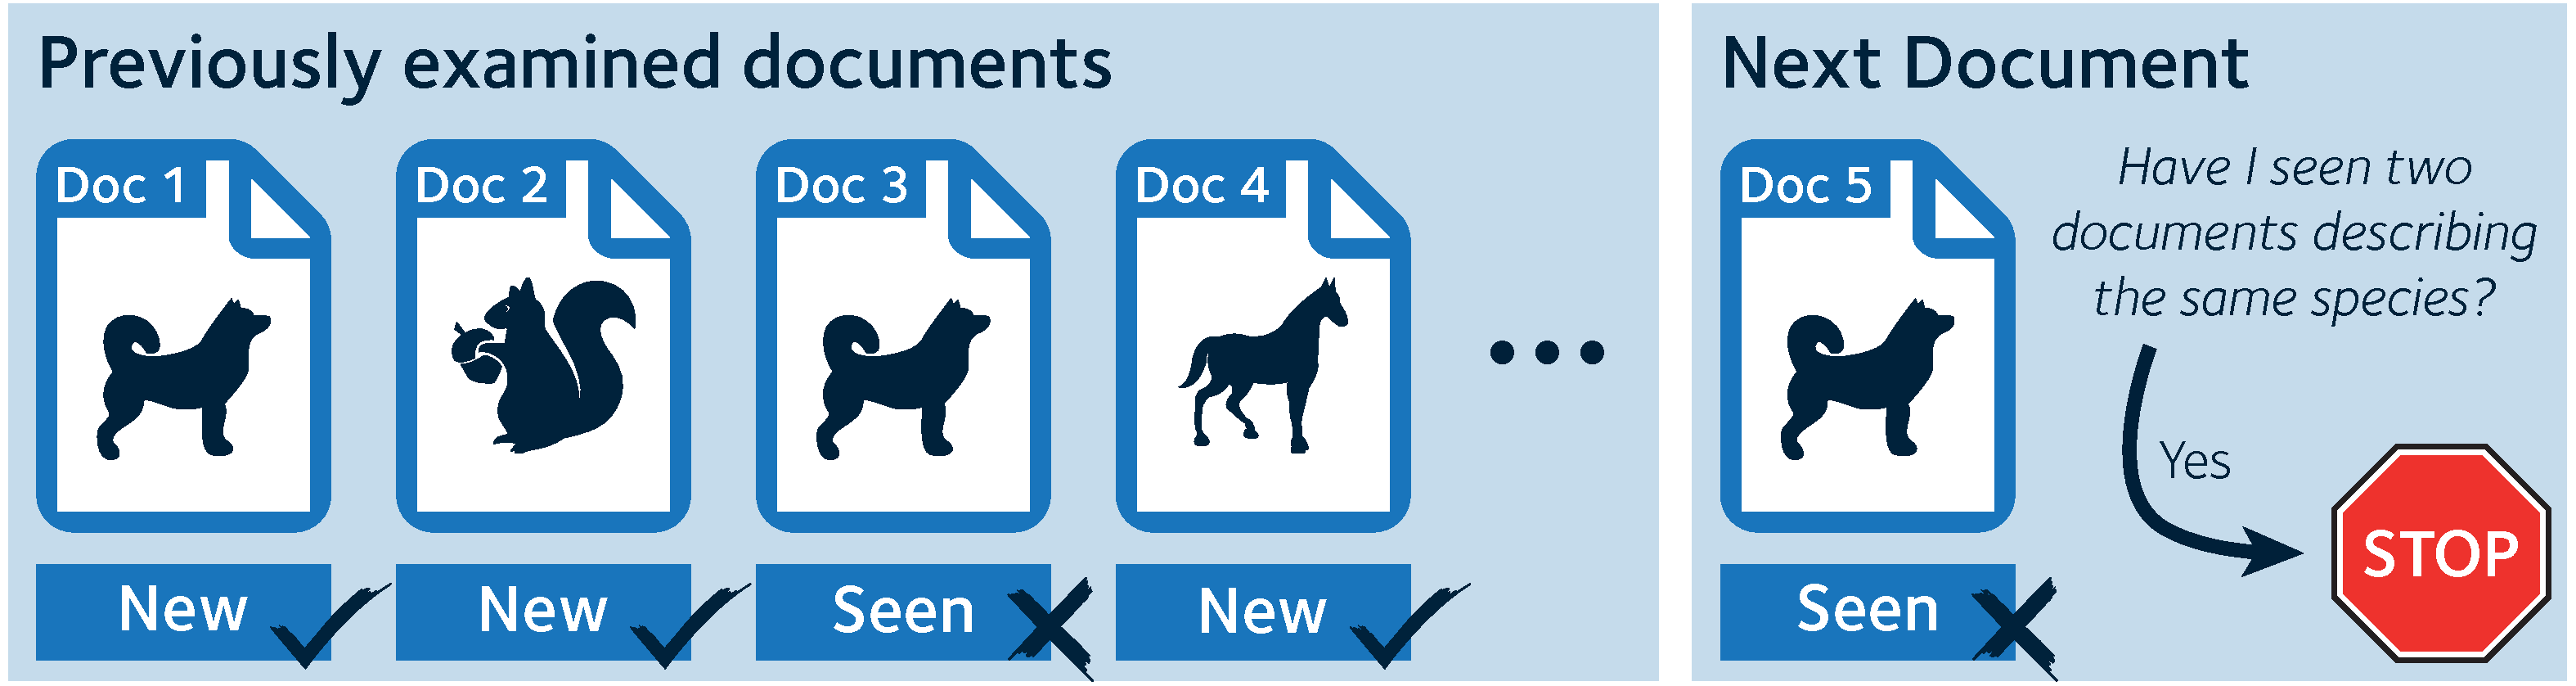
\includegraphics{figures/ch3-difference.pdf}}
    \caption[Difference threshold heuristic]{A simplified example of the difference threshold heuristic. Given the information need of finding different species of animal, a searcher issues a query, and examines a number of documents. The third document offers information on dogs, which has been already observed in \genericblack{Doc 1.} Using the stopping criterion that once the same species has been observed twice, \genericblack{Doc 5} satisfies it. This then means that the threshold has been met, and the searcher then stops.}
    \label{fig:difference_heuristic}
\end{figure}

As a simplistic example of this heuristic, a searcher is provided with an information need to find as many different species of animal as possible. Once a query has been issued, the searcher begins to examine documents on the~\gls{acr:serp}. This is illustrated in Figure~\ref{fig:difference_heuristic}, where the first document considers dogs. A simple criterion is employed whereby the searcher stops after encountering the same animal twice, illustrating that nothing new is being learnt from the list of results presented. Once this is met, the searcher abandons the~\gls{acr:serp}, and can then perform a query reformulation to discover different species of animal.

\subsubsection{Magnitude Threshold}\label{sec:stopping_background:heuristics:magnitude}
The magnitude threshold heuristic~\citep{nickles1995judgment} considers an individual's belief that the information accrued during the search process provides \emph{sufficient evidence} to prompt him or her to stop searching for further information. The point at which the searcher would decide to stop (stopping criterion) is determined by some predetermined, internal threshold that must be reached~\citep{wald1948sequential_analysis, nickles1995judgment}.~\cite{gettys1979hypothesis} hypothesised that the searcher \emph{``mentally tabulates''} the cumulative impact of the evidence that he or she has uncovered. When the tabulation crosses the predetermined threshold, he or she stops.

\begin{wrapfigure}[11]{r}{0.45\textwidth}
    \begin{center}
    \vspace*{-5mm}
    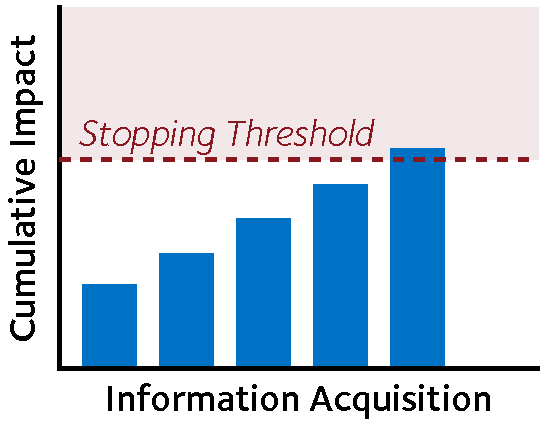
\includegraphics[width=1\textwidth]{figures/ch3-threshold.pdf}
    \end{center}
    \vspace*{-6mm}
    \caption[The magnitude threshold stopping heuristic]{The magnitude threshold heuristic. Once a searcher accrues a predetermined level of impact, he or she stops. Adapted from~\cite{browne2004stopping_rules}.}
    \label{fig:threshold}
\end{wrapfigure}

Determining what exactly this threshold should be before commencing a task has attracted research from several perspectives. This decision can be left open to interpretation by the individuals who choose to operationalise such a heuristic. However, research has shown that under different tasks, varying the criteria by which an individual bases their initial threshold value differs. For example,~\cite{busemeyer1982choice_behaviour} demonstrated this for decision making under uncertainty.~\cite{saad1996stopping} demonstrated the usefulness of this heuristic under common choice tasks. Considering prior knowledge of a topic may also impact upon the threshold chosen -- a topic where a searcher has limited knowledge may mean a lower stopping threshold, for example.

An abstract representation of the stopping heuristic is provided in Figure~\ref{fig:threshold}. From the figure, we can see that a searcher accrues information through each document that is examined. This is combined together to form a \emph{cumulative impact} of the information. For each document examined, the current cumulative impact value is compared against a predetermined threshold value. If the cumulative impact is above this threshold, the searcher then assumes that enough supporting evidence has been collected, and stops.

\subsubsection{Single Criterion}\label{sec:stopping_background:heuristics:single}
The \emph{single criterion heuristic} was later defined by~\cite{browne2005stopping_rules}. As the name suggests, this heuristic considers a searcher examining information for a \emph{single criterion} related to their information need, typically assumed to be the most important one. The searcher then stops examining content once he or she has deduced that enough information about said criterion has been accumulated for them to be satisfied. The concept of a stopping threshold can be borrowed from the magnitude threshold heuristic, discussed in Section~\ref{sec:stopping_background:heuristics:magnitude}. This considers that a searcher will stop once they have accumulated enough impactful information to satisfy their information need.

\cite{browne2005stopping_rules} go on to outline an example search task where the single criterion threshold would be directly applicable. Their example considers purchasing a mortgage for a new house. Here, a searcher will explore the websites of various mortgage lenders in order to find the best deal for them. Given a mortgage deal, the most obvious criterion that an individual would look for would be interest rates. More attractive deals would be associated with lower interest rates. Of course, other factors may influence the decision, but this example ultimately demonstrates how the heuristic works in simplistic terms.

\subsection{Reasoning-Based Heuristics}\label{sec:stopping_background:heuristics:reasoning}
The second category of stopping heuristics as defined by~\cite{nickles1995judgment} are \emph{reasoning based}. While searching and accruing information about a particular topic, a searcher is essentially developing a mental representation of the topic~\citep{yates1990decision_making}. As highlighted by~\cite{nickles1995judgment}, these elements can include arguments constructed during informal reasoning, previously constructed arguments, or information evoked from the searcher's long-term memory. As such,~\cite{nickles1995judgment} devised a category of stopping heuristics that are dominated by the searcher's reasoning processes.

\subsubsection{Representational Stability}\label{sec:stopping_background:heuristics:representational}
The representational stability heuristic~\citep{nickles1995judgment} (with the phenomenon initially discussed by~\cite{yates1982toward}) concerns the notion that as a searcher acquires new information, his or her mental model of the underlying information need shifts and develops -- but only up to a certain point. From this point, their mental model \emph{stabilises,} and the searcher is said to have accrued enough information to satisfy or understand the (sub)topic.

\begin{wrapfigure}[8]{r}{0.45\textwidth}
    \begin{center}
    \vspace*{-6mm}
    
\includegraphics[width=1\textwidth]{figures/ch3-representational.pdf}
    \end{center}
    \vspace*{-5mm}
    \caption[Representational stability stopping heuristic]{Example illustration of the representational stability stopping heuristic. The searcher's model of the given information need begins to stabilise at \emph{t-1}, meaning that a searcher would stop at \emph{t}.}
    \label{fig:representational_heuristic}
\end{wrapfigure}

It is stated by~\cite{nickles1995judgment} that while a searcher examines content, he or she generates arguments that serve to develop and elaborate his or her conception of the decision(s) that they are tasked to make. As the searcher continues to reason, certain arguments may be relegated to long-term memory due to the limited size of the searcher's working memory. Searchers will accrue new information, with some perhaps returning to the original subset of arguments. As mentioned previously, it is this point that can be interpreted as a form of stability regarding the searcher's mental model of their information need. This is depicted in Figure~\ref{fig:representational_heuristic}, where given a vague information need, a searcher will trawl a series of documents in order to develop their mental model of the given problem, turning their understanding of the topic from an initial \emph{fuzzy} state to \emph{crystal clear.}

\vspace*{-4mm}
\subsubsection{Propositional Stability}\label{sec:stopping_background:heuristics:propositional}
Similar to the representational stability heuristic,~\cite{nickles1995judgment} also defined the \emph{propositional stability} heuristic which again focuses on the concept of a stabilising mental model of the given information need. Here, a searcher when examining content will form a series of arguments from the information he or she is observing. These arguments can lead to \emph{tentative conclusions}, from which at some point stability is achieved -- and the conclusion does not change. Therefore, this heuristic suggests that the stabilised nature of the decision maker's conclusion from the information observed prompts him or her to stop.

\vspace*{-4mm}
\subsubsection{The Mental List}\label{sec:stopping_background:heuristics:mental}
The mental list stopping heuristic considers a mental list of aspects of some phenomenon. Each of the different aspects within the mental list must be \emph{`checked off'} to a satisfactory level before the searcher then decides to stop examining content. This mental list can typically be constructed from a searcher's long-term memory, meaning that they will likely have \emph{a priori} knowledge of the particular information need. So-called belief structures such as \emph{schemas}~\citep{bartlett1933remembering} or \emph{scripts}~\citep{schank1977scripts} may assist the searcher in organising the construction of the mental list that forms the set of criteria that determines when they stop.

Figure~\ref{fig:mental_list} provides a graphical illustration of the mental list heuristic. When looking for a new car, a searcher will construct a mental list of different aspects of a car which are essentially the minimum requirements (e.g. a minimum engine displacement of 1.8 litres). Searching is then conducted, with the searcher narrowing down the potential choices available to them to those that satisfy their mental list.

\begin{figure}[t!]
    \centering
    \resizebox{1\hsize}{!}{
    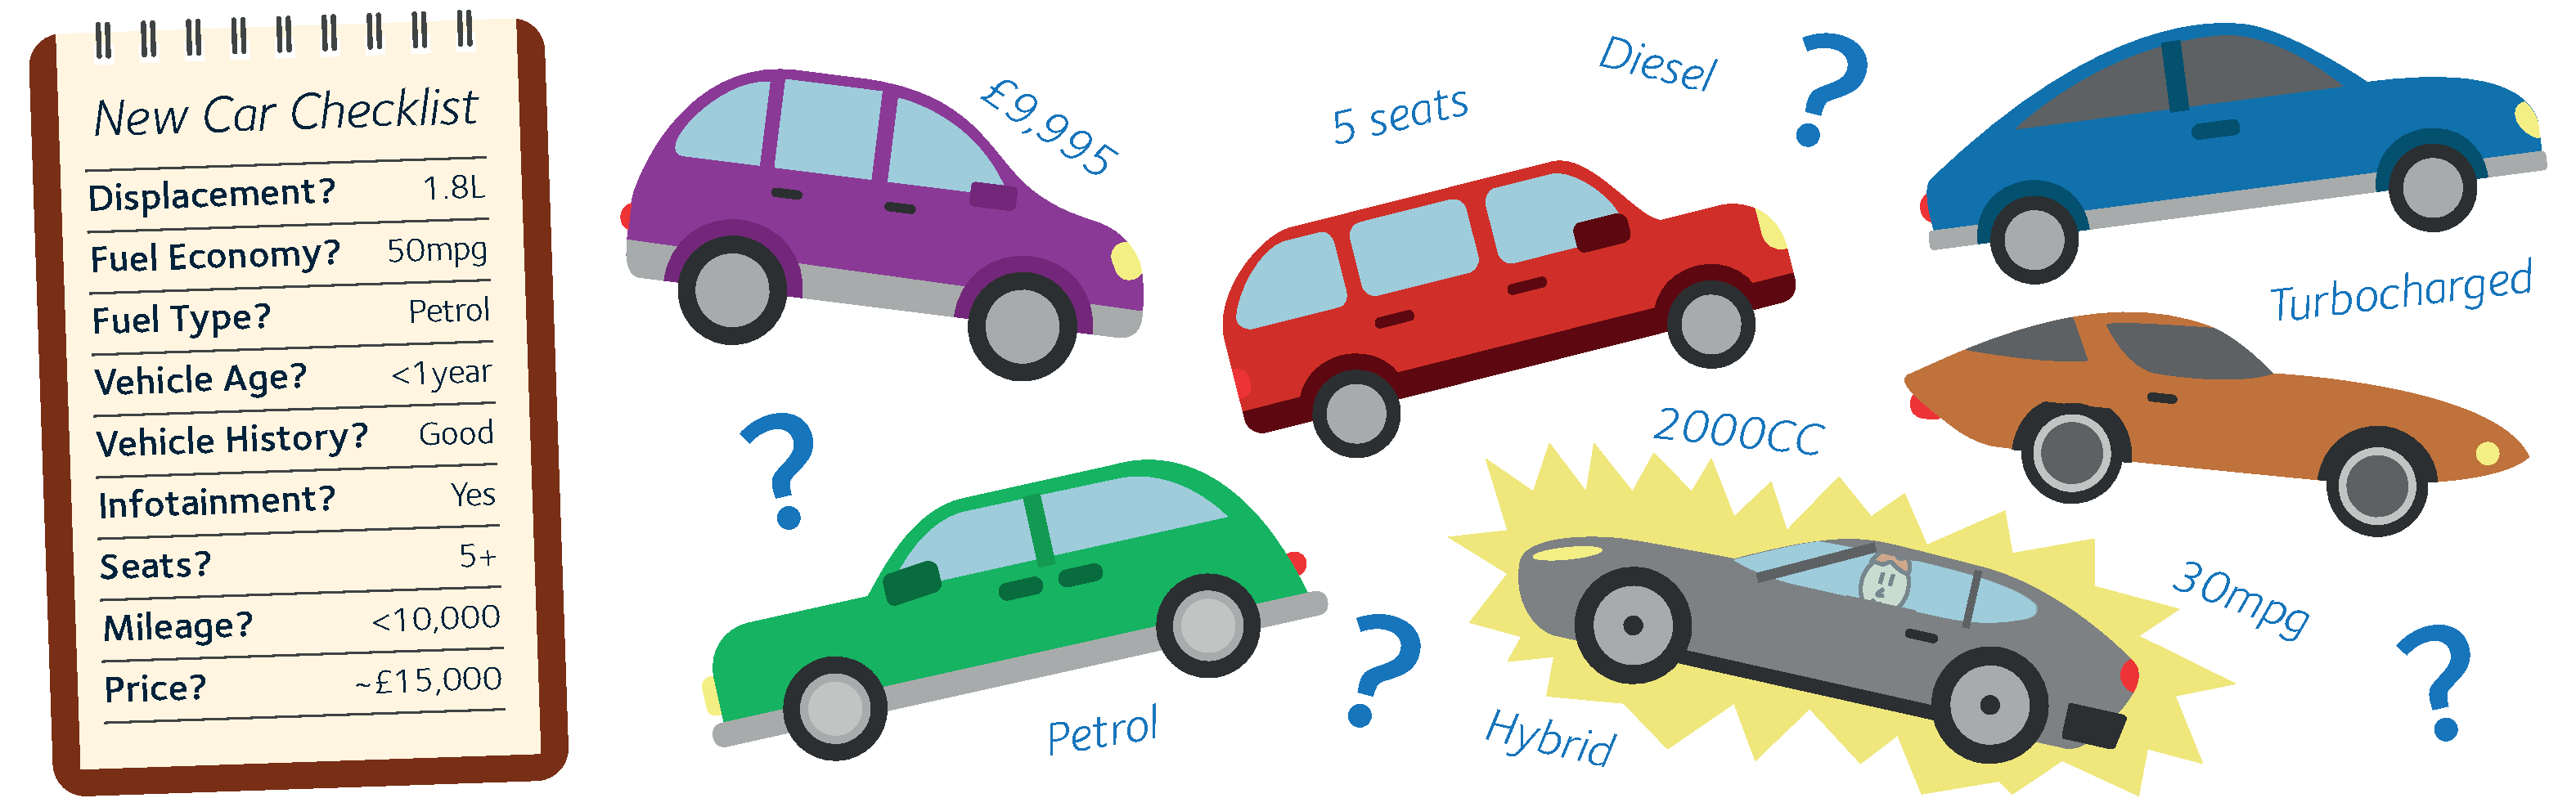
\includegraphics{figures/ch3-mental_list.pdf}}
    \caption[The mental list stopping heuristic]{Given a well defined information need,~\cite{nickles1995judgment} outlined the mental list heuristic, where a number of different criteria must be satisfied before stopping. In the illustration above, car shopping is used as an example. Here, certain criteria for a new car (as shown on the notepad) must be met before a searcher is satisfied with what they have found.}
    \label{fig:mental_list}
\end{figure}

\subsection{Summary of Heuristics}
In this section, a number of different stopping heuristics have been discussed from a number of seminal papers in the literature. While a much larger number of normative stopping heuristics have been defined in prior works, these have been omitted from the review as they do not adequately describe the cognitive behaviours of a searcher, often assuming a searcher has to \emph{think ahead} to make a decision to stop or continue~\citep{browne2004stopping_rules}. In contrast, the heuristics that are enumerated above do not make this assumption, making more realistic assumptions about the searcher's cognitive abilities.

Of course, the different stopping heuristics discussed above are likely to behave differently under different search contexts. As an example, the mental list heuristic might be impossible to use given a searcher with a very limited knowledge of a topic. He or she simply would not know enough information to ascertain key aspects of the topic and construct a set of criteria that must be met~\citep{browne2005stopping_rules} --~\cite{gigerenzer1999betting} also discuss this reasoning for the single criterion stopping heuristic. As such, it is hypothesised that the aforementioned stopping heuristics would likely work better with a searcher who is more knowledgeable.

%Indeed,~\cite{browne2005stopping_rules} hypothesises that magnitude threshold and mental list heuristics would be best applied to searchers with a greater degree of understanding of the topic.

\cite{browne2005stopping_rules} also discuss the so-called \emph{``structuredness''} of a given search task. If the task has well-defined inputs and outputs -- or the goals and operations are clear and easily understood~\citep{simon1996sciences} -- then it is hypothesised that searchers will employ more precise stopping heuristics for deducing when to stop. For example, the mental list and single criterion stopping heuristics might offer greater degrees of precision than (for example) the frustration and satisfaction heuristics, although the frustration and satisfaction heuristics may perform well for any given search task. Altogether, the heuristics discussed in this section would be applicable for informational search tasks~\citep{browne2005stopping_rules} such as ad-hoc retrieval (refer to Section~\ref{sec:ir_background:paradigms:trec}).

With the heuristics now enumerated, we later in this thesis discuss how we take these stopping heuristics and consider how to \emph{operationalise} them, such that they can be subsequently implemented and compared against each other empirically. This also involves which of the two stopping decision points we discussed in Section~\ref{sec:stopping_background:why:points} these operationalised heuristics can be used in. Chapter~\ref{chap:strategies} provides explanations of the twelve \emph{stopping strategies} that we employ in the contributory work in this thesis.

\section{Theoretical Models}\label{sec:stopping_background:theoretical}
In addition to the stopping heuristics above, mathematically grounded, theoretical models have been defined that allow us to describe, predict and explain \emph{how} and \emph{why} searchers behave in the way they do. Crucially for this thesis, such models provide an explanation of their stopping behaviour. As discussed in Section~\ref{sec:ir_background:user:simulation} however, such models also have limitations, ranging from the low-level assumptions engaged by the different models, the variables that are considered or excluded from the models, and the difficulties arising from the complexities of human behaviour~\citep{fishwick1995simulation, azzopardi2015theories}.

Despite the limitations of such an approach, such \emph{formal models} also permit the generation of different hypotheses regarding search behaviours. These can subsequently be empirically tested and validated -- with examples of such studies including~\cite{azzopardi2013query_cost} and~\cite{pirolli1996scatter_techniques}. Three examples of such theories include~\glsfirst{acr:ift}~\citep{pirolli1999ift},~\glsfirst{acr:set}~\citep{azzopardi2011economics} and the~\glsfirst{acr:iprp}~\citep{fuhr2008iprp}. Central to the work in this thesis is~\gls{acr:ift} that we discuss in detail in the following subsection. As shown by~\cite{azzopardi2015theories} however, the three theories are all mathematically equivalent, with all ultimately leading to the same understanding. As such, we do not discuss~\gls{acr:set} and~\gls{acr:iprp} in detail.

%As such, this section focuses on a discussion of~\glsfirst{acr:ift} as a means for explaining a searcher's \emph{optimal stopping behaviour.} We also briefly acknowledge two other competing theoretical models of search.

\subsection{Information Foraging Theory}\label{sec:stopping_background:theoretical:ift}
A well known conceptual model in the field of information seeking is the \emph{berry picking model}, as proposed by~\cite{bates1989berry_picking}. As shown in Figure~\ref{fig:berry_picking}, this model considers searchers looking for information to be analogous to \emph{foragers} scavenging for food in the wild. In the model, foragers are looking for the juiciest and ripest berries on a number of different bushes (or \emph{\glsplural{glos:patch}}). The juiciest and ripest berries offer the highest levels of gain. Picking these berries helps the forager maximise their level of gain. Applied to search, this construct means that a searcher \emph{forages for information,} picking the most relevant (or juiciest!) documents that help them maximise their level of gain.

\begin{figure}[t!]
    \centering
    \resizebox{1\hsize}{!}{
    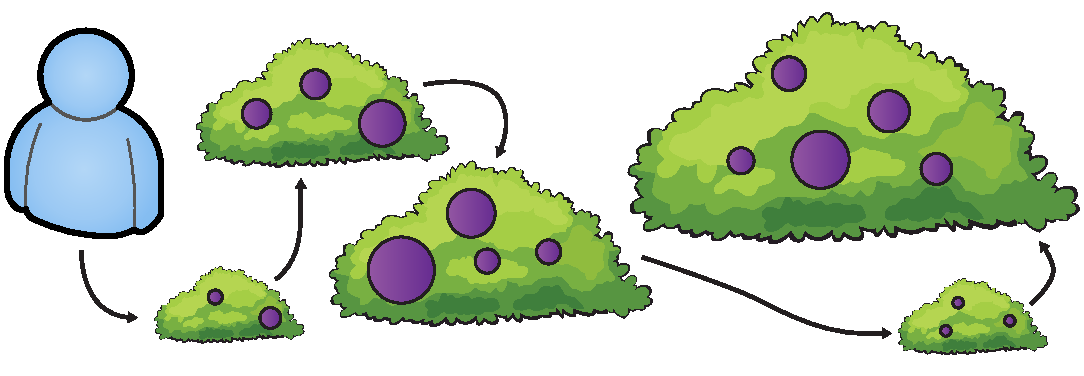
\includegraphics{figures/ch3-berry_picking.pdf}}
    \caption[The Berry Picking Model~\cite{bates1989berry_picking}]{The \emph{Berry Picking Model}~\cite{bates1989berry_picking}. A forager traverses through bushes to pick the juiciest berries for consumption. The model is high level and conceptual in nature, and thus does not provide any justification for \emph{how} or \emph{why} foragers search for the juiciest berries.}
    \label{fig:berry_picking}
\end{figure}

While the berry picking model is an intuitive and simple model to understand, its highly descriptive nature does not provide an explanation regarding the behaviour of the forager. \emph{How long should a forager spend examining this berry bush?} This question cannot be answered as such by the model, but~\cite{bates1989alluding} in a later publication does allude to the fact that searchers could weigh up the costs and benefits in order to decide what to do next.

Theories do however exist that attempt to explain the behaviour of a searcher when \emph{foraging} for information. Initial attempts by~\cite{russell1993sense_making} and~\cite{sandstrom1994optimal_foraging} demonstrated that~\glsfirst{acr:oft}~\citep{stephens1986foraging_theory} could be potentially used to model the search process. This led to the development of~\glsfirst{acr:ift}, proposed by~\cite{pirolli1999ift}. The theory provides an explanation as to how information foragers will behave, and as such, also provides a rationale as to how they will stop.~\gls{acr:ift} is extensively used in this thesis as a theoretical underpinning to several hypotheses. We also outline an optimal stopping heuristic, as well as several other time-based heuristics that derive from work associated with~\gls{acr:oft}.

\subsubsection{Patches and Scent}\label{sec:stopping_background:theoretical:ift:patch}
\gls{acr:ift} is comprised of three main models: the \emph{information diet model}, concerning \emph{what} information is consumed; the \emph{information patch model}; and the \emph{information scent model.} With the information diet model not considered in this thesis, we focus in this section on discussing the information patch and information scent models.

Central to~\gls{acr:ift} is the notion of a \emph{patch}, as per the patch model. In the wild, a patch is modelled as an area of land with a degree of potential gain (food) that can be acquired by foraging through the said patch. The \emph{between patch time} is the amount of time a forager spends moving towards a patch, and the \emph{within patch time} is the time spent within the patch, examining its contents for potential gain.

With~\gls{acr:ift}, a patch can be modelled in a variety of ways. However, as outlined by~\cite{azzopardi2015theories}, the generally agreed approach to model a patch in terms of information seeking is to consider it as a~\gls{acr:serp}. With this representation, moving between a patch is akin to \emph{issuing a query,} and thus incurs a cost. This is called the \blueboxbold{between patch time}. Staying within a patch is the same as assessing result summaries on the presented~\gls{acr:serp} and their associated documents, with each summary and/or document taking a certain amount of time to process, or the \blueboxbold{within patch time}. The patch model essentially predicts how long an information forager should stay in a patch (or~\gls{acr:serp}) before abandoning it and moving to the next patch.

However, given a series of patches (or potential queries), how does a forager deduce which one they should \emph{enter next,} and examine in closer detail? This is described by the information scent model and encapsulates a currently active area of research. Figure~\ref{fig:patch_model} graphically illustrates the scent of a patch in action -- given two patches as depicted in the illustration, which patch will the forager travel to next? Following the scent or \emph{cues} on the ground next to him, the forager observes that the paw prints to patch \raisebox{-.2\height}{
\includegraphics[height=5mm]{figures/ch2-point1.pdf}} are more prevalent, and thus will venture to that patch first. Like foragers in the wild, information foragers will observe a series of \emph{proximal cues} presented to them on a~\gls{acr:serp}, such as hypertext links, document titles, snippet text and thumbnails to locate information~\citep{pirolli1995ift, pirolli1999ift, chi2001information_scent, oltston2003scenttrails, pirolli2007ift}. In the context of news search, cues were examined by~\cite{sundar2007news_scent}. Here, cues such as the source of an article (its scent) were shown to have a powerful effect on the perception of the article, and influenced whether the said article was clicked on.

If these cues provide a rationale as to what leads to a promising scent trail, it follows that scent, in combination with patches, provides a rationale as to when a searcher will stop examining a set of results~\citep{pirolli1999ift, wu2012dc, wu2014information_scent}. For example, a user study by~\cite{wu2014information_scent} demonstrated that a searcher would forage to greater depths if the~\gls{acr:serp} appeared to contain many relevant items.~\cite{card2001scent_graphs} also observed this trend. They found that when navigating through pages, searchers were more likely to leave when the information scent began to decline. Section~\ref{sec:stopping_background:user_studies} provides more details on these user studies, along with others considering stopping behaviours.

\begin{figure}[t!]
    \centering
    \resizebox{1\hsize}{!}{
    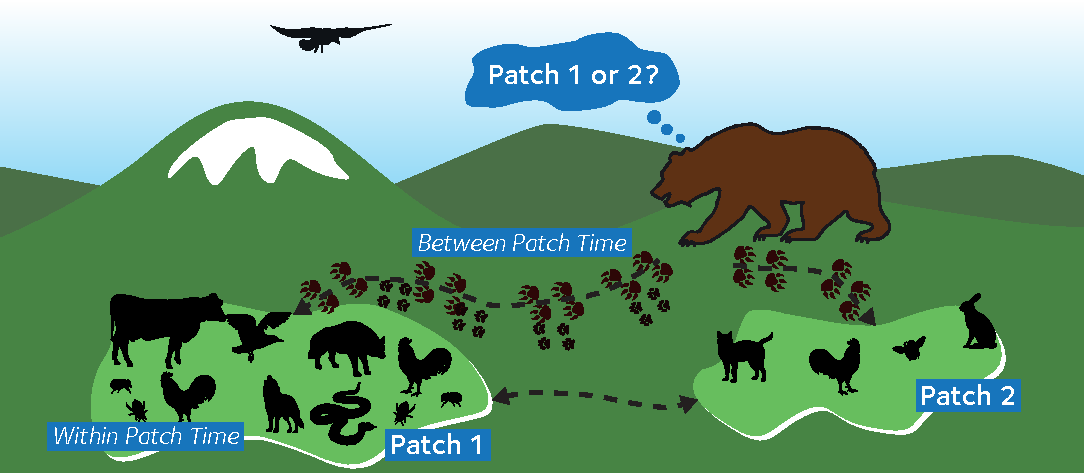
\includegraphics{figures/ch3-patch.pdf}}
    \caption[The patch model]{A graphical depiction of the \emph{patch model}, part of ~\glsfirst{acr:ift}. When presented with two patches, each containing food that can be represented as gain, what patch should our forager choose first — patch \raisebox{-.2\height}{
\includegraphics[height=5mm]{figures/ch2-point1.pdf}} or \raisebox{-.2\height}{
\includegraphics[height=5mm]{figures/ch2-point2.pdf}}?}
    \label{fig:patch_model}
\end{figure}

\subsubsection{Stopping Heuristics}\label{sec:stopping_background:theoretical:ift:stopping}
Given a patch with a scent, how can one deduce \emph{when they should stop?} Like all theories,~\gls{acr:ift} makes some key assumptions from which we can deduce behaviours of a forager. The assumptions are that a forager will: enter a patch with what appears to be the highest yield first; and attempt to maximise their gain per unit of time. Given these assumptions, one would now be able to answer the question posed in Figure~\ref{fig:patch_model}. With a better scent and greater volume of potential energy to be gained, patch \raisebox{-.2\height}{
\includegraphics[height=5mm]{figures/ch2-point1.pdf}} is the answer that a forager would provide to the question \emph{which patch should I explore first?}

% \begin{itemize}
%     \item{enter a patch with what appears to be the highest yield first; and}
%     \item{attempt to maximise their gain per unit of time.}
% \end{itemize}

In addition, the assumptions provided above allow us to begin formulating a stopping heuristic based on the \emph{optimal behaviour} of a forager. The~\gls{acr:mvt} by~\cite{charnov1976mvt} states...

\begin{quote}
    \emph{``...that a forager should remain in a patch so long as the slope of the gain function is greater than the average rate of gain in the environment.''}
    \attrib{\cite{pirolli1999ift}}
\end{quote}

\begin{wrapfigure}[11]{r}{0.45\textwidth}
    \begin{center}
    \vspace*{-11mm}
    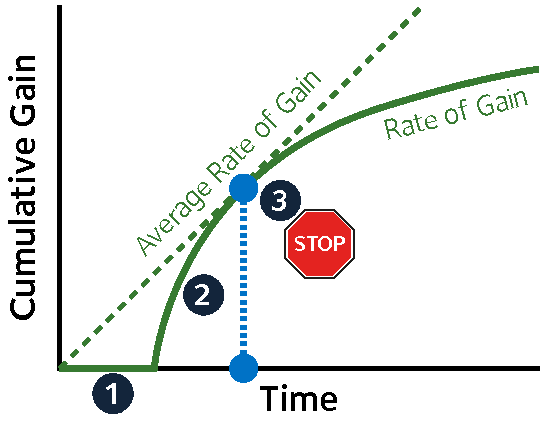
\includegraphics[width=1\textwidth]{figures/ch3-ift_stop.pdf}
    \end{center}
    \vspace*{-6mm}
    \caption[Optimal \gls{acr:ift} stopping heuristic]{The~\gls{acr:ift} stopping heuristic. The searcher should stop when the rate of gain (solid \textbf{\color{dmax_green}green} line) no longer outperforms the average rate of gain (dotted \textbf{\color{dmax_green}green} line).}
    \label{fig:ift_stopping}
\end{wrapfigure}

The~\gls{acr:mvt} implies that if a forager is within a patch that initially looked promising, yet is yielding a rate of gain less than the \emph{average rate of gain expected within the patch,} he or she should then abandon the patch and then move to another one. This phenomenon is often called the \emph{instantaneous intake} theorem~\citep{stephens1986foraging_theory}. In the context of information seeking, this would imply a query reformulation. Conversely, a forager who has found himself or herself in a patch yielding gain at a rate \emph{greater} than the average rate of gain would be best advised to stay within that patch. This is graphically illustrated in Figure~\ref{fig:ift_stopping}, where the \emph{gain curve} for a forager in a patch is highlighted in \genericblack{\color{dmax_green}green}. In addition, the plot illustrates: \raisebox{-.2\height}{
\includegraphics[height=5mm]{figures/ch2-point1.pdf}} the between patch time, where the forager is not acquiring any gain; \raisebox{-.2\height}{
\includegraphics[height=5mm]{figures/ch2-point2.pdf}} the within patch time, where the forager is examining the~\gls{acr:serp} and associated documents; and \raisebox{-.2\height}{
\includegraphics[height=5mm]{figures/ch2-point3.pdf}} the optimal stopping point, based upon the~\gls{acr:mvt}. Graphically, this is best described as the point at which the tangent to the curve (from the origin) touches the gain curve. From this point onwards, the rate of gain decreases and is less than the average rate of gain, meaning that the forager receives diminishing returns for the investment in examining content within the current patch (or~\gls{acr:serp}).

\begin{figure}[t!]
    \centering
    \resizebox{1\hsize}{!}{
    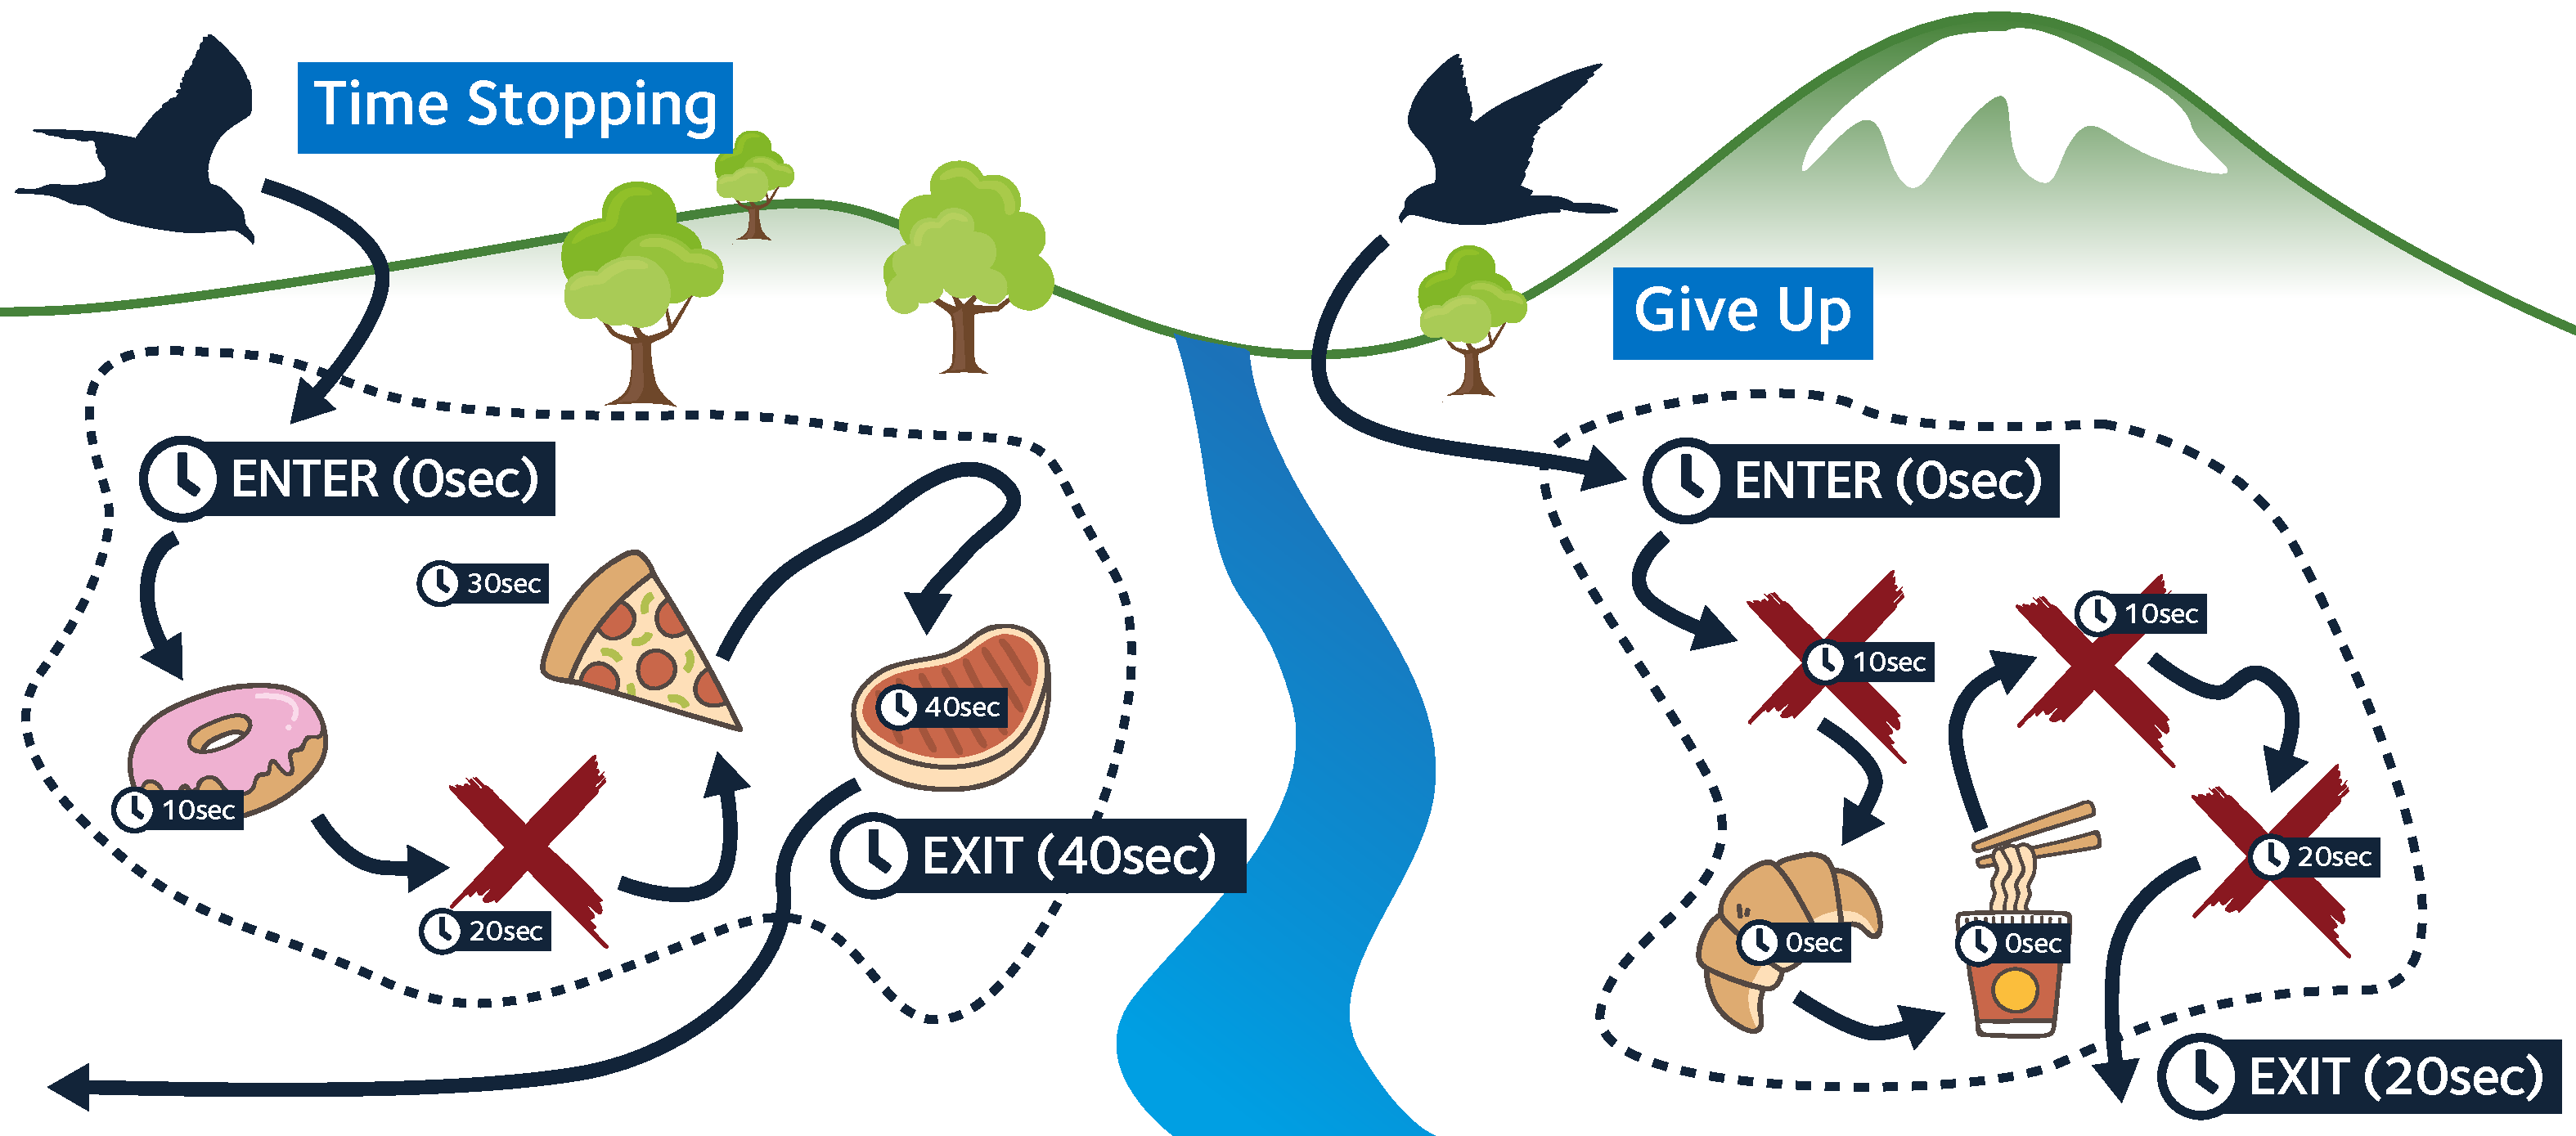
\includegraphics{figures/ch3-gut.pdf}}
    \caption[Time-based stopping heuristics]{Illustrations of the \emph{time stopping heuristic} (left), and the \emph{give up heuristic} (right). On the left, a forager will stop after a time limit has been reached (40 seconds in this example) from the point at which they enter a patch. On the right, a forager will \emph{reset} their timer when they encounter something gainful, but will grow increasingly impatient the poorer the results of their foraging, and eventually stop too (a 20 second limit is shown here).}
    \label{fig:gut}
\end{figure}

Operationalising the instantaneous intake theorem is often difficult to do in practice. How would one measure, for example, the expected rate of gain? Instead, several other stopping heuristics that influence patch leaving have been developed as part of~\gls{acr:oft}~\citep{stephens1986foraging_theory}. These attempt to approximate the instantaneous intake theorem. Such heuristics include, but are not limited to:

\begin{itemize}
    \item{the so-called \blueboxbold{number heuristic}~\citep{gibb1958number_rule}, where a forager would leave a patch after finding $n$ prey;\footnote{This stopping heuristic is analogous to the satisfaction and satiation stopping heuristics, defined by~\cite{cooper1973retrieval_effectiveness} and~\cite{simon1955satiation} respectively.}}
    
    \item{the \blueboxbold{time heuristic}~\citep{charles1972behaviour, krebs1973time_rule}, where a forager stops after spending $x$ seconds within a patch; and}
    
    \item{the \blueboxbold{give up} heuristic~\citep{krebs1974leave_after_rule}, where a forager would stop and leave a patch after $x$ seconds have elapsed since last finding something of use.}
\end{itemize}

The time-based stopping heuristics are illustrated in Figure~\ref{fig:gut}. A further study of different \emph{patch types} (i.e. where the density of prey varies) was also undertaken by~\cite{mcnair1982gut_mvt}. They found that across different patch types, different stopping heuristics worked better in different environments -- also demonstrated in works by~\cite{iwasa1981prey_distribution},~\cite{mcnair1982gut_mvt} and~\cite{green1984oft_stopping}. Consequently, a further \blueboxbold{combination heuristic} was devised. For a patch that appears to be fruitful early on, a satisfaction-based heuristic would perform well. Otherwise, employing the give up time-based heuristic~\citep{krebs1974leave_after_rule} would work best. This intuitively makes sense. A searcher, when presented with a~\gls{acr:serp} of high quality with many relevant results would be prudent to continue examining it for more content if the initial set of results are promising. However, if initial results are not promising, the searcher should be more sceptical, and be prepared to abandon it if, after examination, relevant content was not forthcoming as the results are traversed.

%In other words, a searcher should stop when the marginal gain equals the marginal cost of examining the results.

% \subsection{Other Theoretical Models of Search}\label{sec:stopping_background:theoretical:other}
% It is important to acknowledge that apart from~\gls{acr:ift}, other competing theoretical models of search exist and are being actively developed. The two competing models are~\glsfirst{acr:set}~\citep{azzopardi2011economics} and the~\glsfirst{acr:iprp}~\citep{fuhr2008iprp}. These models have both been shown to be mathematically similar to~\gls{acr:ift} in terms of explaining searcher behaviours -- as shown by~\cite{azzopardi2015theories} -- and as such we limit discussion of these two theoretical models to a brief overview.
%
% As the name suggests,~\gls{acr:set} concerns the modelling of the search process by addressing it as an economics problem, using \emph{production theory}~\citep{varian1987intermediate}. In production theory, a \emph{output} is produced by a firm (goods or services), but requires \emph{input} (capital or labour). The intermediary process employs some form of \emph{technology} to produce the given goods, or to provide the service. In the context of the search process, this maps to the following two inputs:
%
% \begin{itemize}
%     \item{$Q$, the number of \emph{queries} that a searcher will issue; and}
%     \item{$E$, the number of documents that the searcher will \emph{examine} per query.}
% \end{itemize}
%
% Output is considered as the amount of gain that a searcher extracts from the relevant documents that are found. These can be then combined to create \emph{gain functions} (i.e. $g(Q,E)$) and \emph{cost functions} (i.e. $c(Q,E)$). From these, different hypotheses can be generated, as used by~\cite{azzopardi2013query_cost}, and demonstrated in Section~\ref{sec:stopping_background:user_studies:depths}.
%
% The second theoretical model is the~\gls{acr:iprp}. Essentially, the~\gls{acr:iprp} forms an extension to the~\glsfirst{acr:prp}~\citep{robertson1977prp}, but relaxed a number of modelling assumptions made by the~\gls{acr:prp}, namely:
%
% \begin{itemize}
%     \item{the notion of a fixed information need; and}
%     \item{the relevance of a document is independent of previously seen documents.}
% \end{itemize}
%
% While these approximations do offer reasonable assumptions, they have been shown to break down in the past~\citep{gordon1991utility_theory}. The high level, generalisable~\gls{acr:iprp} accounts for different costs and benefits that are associated with particular \emph{situations} and \emph{choices} when ranking a series of documents.


\section{User Studies}\label{sec:stopping_background:user_studies}
While stopping heuristics provide a means for quantitatively characterising and predicting stopping behaviour~\citep{wu2014information_scent}, only a handful of user studies have been undertaken that attempt to understand when enough information is enough~\citep{zach2005enough_is_enough}. As we have already discussed, stopping is an inherently difficult phenomenon to model effectively. This is because it is instrumented by a series of internal factors to the decision maker's thinking~\citep{nickles1995judgment}. In this section, we detail a number of different user studies that have attempted to provide an explanation for a searcher's stopping behaviours.

\subsection{Understanding Stopping Behaviours}
Two user studies by~\cite{zach2005enough_is_enough} and~\cite{berryman2006defines} have examined searcher stopping behaviours through a series of interviews with subjects. These studies primarily focused on the notion of \emph{why} searchers stopped when they did, with both considering subjects seeking information in an academic work environment.

\cite{zach2005enough_is_enough} considered how senior art administrators determined when to stop searching in their daily jobs, and found that they mostly stopped either because they:

\begin{itemize}
    \item{felt satisfied with the information that they had obtained during their search; or}
    \item{stopped because of time constraints.}
\end{itemize}

The study by~\cite{berryman2006defines} was conducted in a similar approach. Public sector policy workers reported finding it difficult to work out how much information would be enough to satisfy their tasks when initiating them. However, once the structure of what they needed to find had been established, the point at which they felt they should stop became clearer. The findings from this second study provide evidence that the assessments of what constitutes as \emph{enough} can be difficult and complex to deduce. This finding also provides evidence of the development of an underlying mental model of the given information need and provides justification for the representational stability, propositional stability, and mental list stopping heuristics (as discussed in Section~\ref{sec:stopping_background:heuristics:reasoning}).

A number of user studies have also examined stopping behaviours in relation to the concept of satisfaction or satiation~\citep{simon1955satiation}. As previously discussed in Section~\ref{sec:stopping_background:heuristics:frustration}, this concept suggests that a searcher will cease searching as soon as conditions arise, instead of after they have exhaustively considered all available information~\citep{march1994primer}.

Considering this approach,~\cite{agosto2002satisficing} examined the decision-making abilities of young people when searching on the~\gls{acr:www}. In this study, 22 9\textsuperscript{th} and 10\textsuperscript{th} grade students from a U.S. high school demonstrated limitations which affected their decision making, including time constraints that were imposed externally and internally, information overload, and other physical constraints. In order to find websites to help in satisfying their information need, the students used reductive approaches to decrease the amount of information presented on the~\gls{acr:www}, and used this to work out when to stop. How students perceived the websites were also largely down to personal preference.

With a completely different set of subjects,~\cite{mansourian2007search} conducted a study where they analysed the stopping behaviours of 37 staff and students from four university biology departments, and classified their stopping behaviours by search depth and search impact. Qualitative results showed that subjects indicated that missing potentially important information in the course of their searching was a matter of concern. The authors reported that the estimations and importance of information missed likely would affect their stopping behaviour. From this, classifications of the perceptions of missing information ranged from \emph{inconsequential} to \emph{disastrous}, and search strategies classified as \emph{perfunctory} to \emph{extensive}, with the information need dictating what category the searcher would have considered appropriate.

A similar study by~\cite{prabha2007enough} considered searchers in a further academic library setting, with one key finding from their study showing that time constraints led to a decrease in the number of documents that searchers examined. Again, the specific information need and the searcher's role in academia affects every stage of their search processes -- which includes affecting what they have found to be enough.

These findings were further demonstrated by~\cite{wu2014information_scent}, who undertook a study where subjects performed a series of different search tasks. Subjects were then interviewed about their result summary level stopping and session stopping behaviours. Results from this study showed that result summary level stopping decisions were taken primarily on the face of search results, queries and search tasks. Session stopping decisions were determined by the subject's overall goal for each task, the content examined (and their subjective perceptions of the examined content) and the study constraints imposed upon them, such as time constraints and search interface restrictions. Further empirical evidence to this study was later provided by~\cite{wu2014stopping_query_abandonment}. They reported that some subjects discussed \emph{``forced stopping''} (stopping when no more information could be found), and \emph{``voluntary''} stopping that stemmed from the feeling of securing enough information.

\cite{wu2014information_scent} also discussed how information scent affects the stopping behaviour of a searcher. Constituting part of~\gls{acr:ift}, it is important to note that user studies have been conducted using this model. For example,~\cite{card2001scent_graphs} observed that if a person started with a high information scent web page, he or she would be inclined to visit more web pages on the high scented page's domain. They also found that as the information scent of web pages declined, there was a tendency for the person to leave the site or return to a previously visited page.~\cite{loumakis2011image_smells} examined scent that was associated with images presented on~\glsplural{acr:serp}, and how these impacted on the evaluation behaviour of searchers. They found that when images were added to text snippets, participants reported increased confidence that they could find an appropriate result.\footnote{\emph{A picture is worth a thousand words.}}

Central to the findings of all of the above studies -- regardless of the group of subjects or contexts in which the searches were conducted -- is the idea that searchers stop when they are \emph{satisfied.} Even though subjects of these studies were acutely aware of the fact they had not found \emph{all} relevant information to their given information need, they were nevertheless satisfied with what they had found, and subsequently decided to stop. While the results from these studies may be underwhelming in terms of concrete explanations as to why people stop, they do provide invaluable insights, and demonstrate just how difficult it is to encapsulate or create descriptive parameters of such behaviour. Indeed, factors such as time constraints, a searcher's information seeking ability and other factors all influence the internal stopping rules of a searcher, as was discussed by~\cite{marchionini1995information_seeking}. 

\subsection{Quantifying Stopping Behaviours}
With the above studies examining \emph{why} people decide to stop, a very limited number of studies have attempted to quantify \emph{when} a searcher should stop searching -- something the stopping heuristics presented in Section~\ref{sec:stopping_background:heuristics} attempt to do.~\cite{toms2009predicting_stopping} studied the actions preceding the endpoints in information seeking to predict what actions would lead a searcher to stop. The most prevalent pattern they observed that matches the searcher models outlined in Section~\ref{sec:ir_background:user:models} consisted of a searcher:

\vspace{-5mm}
\begin{itemize}
    \item[\raisebox{-.2\height}{
\includegraphics[height=5mm]{figures/ch2-point1.pdf}}]{issuing a query;}
    \item[\raisebox{-.2\height}{
\includegraphics[height=5mm]{figures/ch2-point2.pdf}}]{examining results presented to them on a~\gls{acr:serp}; and}
    \item[\raisebox{-.2\height}{
\includegraphics[height=5mm]{figures/ch2-point3.pdf}}]{viewing a document.}
\end{itemize}
\vspace{-5mm}

Interestingly, the authors observed that searchers appeared to be more engaged in page content and in revisiting and assessing pages that had already been found. They hypothesised that this again may be due to the satiation heuristic, where the searchers would purposefully go back to reassess if what they had found was \emph{enough.}

A further study by~\cite{dostert2009satisficing} examined the stopping behaviours of 23 undergraduate students. Subjects, in parallel to other studies, reported that the primary factor for deciding to stop was their intuition. Like in the study reported by~\cite{prabha2007enough}, the subjects were time constrained.~\cite{dostert2009satisficing} reasoned that subjects could not adequately articulate this intuition, but hypothesised that they simply felt that given their perception of how much time had elapsed, the number of documents that they had located felt sufficient. However, the authors report a number of additional reasons (as shown in Figure~\ref{fig:stopping_respondents}) why subjects decided to stop, with the reasons providing links back to the stopping heuristics defined in Section~\ref{sec:stopping_background:heuristics}.

\begin{wrapfigure}[13]{r}{0.45\textwidth}
    \begin{center}
    \vspace*{-8mm}
    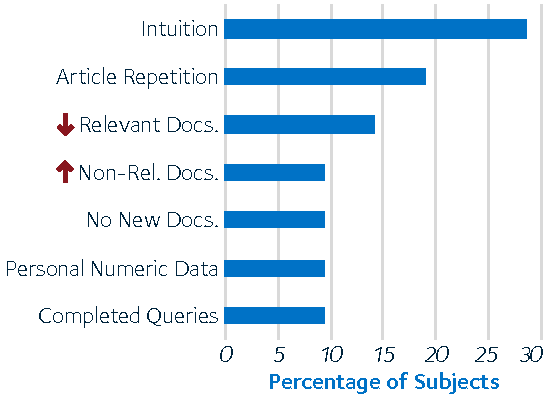
\includegraphics[width=1\textwidth]{figures/ch3-respondents.pdf}
    \end{center}
    \vspace*{-2mm}
    \caption[Responses of a survey by~\cite{dostert2009satisficing}]{Responses of the survey on why subjects stopped by~\cite{dostert2009satisficing}. Like most studies examining stopping behaviour, most subjects stopped because of their \emph{intuition} \textemdash~or what felt like \emph{enough} to them.}
    \label{fig:stopping_respondents}
\end{wrapfigure}

Indeed, the unarticulated notion of finding \emph{``enough''}~\citep{zach2005enough_is_enough} information links neatly back to the idea of the magnitude threshold stopping heuristic, proposed by~\cite{nickles1995judgment} and detailed in Section~\ref{sec:stopping_background:heuristics:magnitude}. With this heuristic, a searcher would stop once they have accumulated a certain predetermined amount of information. From the results of their study,~\cite{dostert2009satisficing} hypothesised that the threshold was reached once their subjects felt they had correctly identified \emph{half} of the relevant documents available to them. In reality, the searchers had on average only managed to correctly identify $7.35\%$. In addition to comparisons to the magnitude threshold stopping heuristic,~\cite{dostert2009satisficing} also drew comparisons from their results to the difference threshold stopping heuristic, as outlined in Section~\ref{sec:stopping_background:heuristics:difference}. To recap, this heuristic considered a searcher's tolerance to not learning anything new. This is argued by the authors as a reason for respondents citing repetition in the documents found, or a lack of new documents. Lastly, the representational stability stopping heuristic as detailed in Section~\ref{sec:stopping_background:heuristics:representational} was also noted by the authors. With this heuristic concerning the stabilisation of the searcher's underlying mental model of the topic, the authors noted that supporting evidence was obtained by subjects responding to a decrease in the number of relevant, and/or an increase in the number of non-relevant documents.

These stopping heuristics were also investigated by~\cite{browne2004stopping_rules} and~\cite{pitts2004stopping_rules} with systems analysts during the process of information requirements determination. The analysts were required to gather a series of information requirements that would allow them to generate diagrams to represent an online grocery shopping system.~\cite{browne2004stopping_rules} found that more experienced analysts tended to use the mental list and magnitude threshold stopping heuristics, while less experienced analysts utilised the difference threshold and representational stability stopping heuristics. In addition to these findings, the authors noted that the applicability of different stopping heuristics resulted in varying degrees of quantity, depth and the quality of information obtained.

\subsection{Considering Search Depths}\label{sec:stopping_background:user_studies:depths}
\begin{wrapfigure}[9]{r}{0.45\textwidth}
    \begin{center}
    \vspace*{-8mm}
    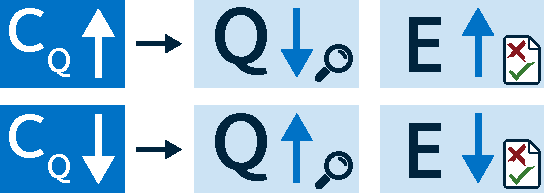
\includegraphics[width=1\textwidth]{figures/ch3-query-cost.pdf}
    \end{center}
    \vspace*{-4mm}
    \caption[The cost-interaction hypothesis]{The \emph{cost-interaction hypothesis}~\citep{azzopardi2011economics}. As the cost of querying increases (\emph{C\textsubscript{Q}}), searchers will issue fewer \textbf{Q}ueries and \textbf{E}xamine more documents per query.}
    \label{fig:query_cost}
\end{wrapfigure}

A number of additional user studies have also considered the so-called \emph{search depth} -- that is, the depth on a list of ranked results that searchers stop clicking (the \emph{click depth}). Studies such as the seminal work by~\cite{cutrell2007eye_tracking} undertook an eye-tracking study and reported that subjects examined the first eight results before deciding to carry out a query reformulation.~\cite{lorigo2008eye_tracking} also examined their subjects' scan paths as they undertook search tasks. On average, subjects scanned only $3.2$ distinct search results per query. This work was supplemented by~\cite{huang2011no_clicks}, where they found that subjects proceeded to issue a new query after inspecting the top four results of the presented~\gls{acr:serp}.

A study by~\cite{azzopardi2013query_cost} also found that the depth to which subjects examined content was affected by the \emph{cost} of entering a query (as illustrated in Figure~\ref{fig:query_cost}). With a search interface where subjects were required to invest more effort to enter a query, significantly fewer queries were issued, with the results for these queries examined to greater depths. This was in contrast to subjects who used a standard search interface, where more queries were issued with subjects examining the content to a shallower depth. These findings comply with the \emph{query-cost hypothesis}~\citep{azzopardi2011economics}, that states: \emph{as the cost of querying increases, searchers will pose fewer queries and examine more documents per query.}

This is illustrated in Figure~\ref{fig:query_cost}. Evidence from this study also demonstrated that the search interface individuals are subjected to impacts upon their stopping decision making.

\section{Chapter Summary}
This chapter has provided an extensive overview of how stopping has been examined in the context of~\gls{acr:iir}. In particular, we have detailed a number of different \emph{stopping heuristics} that have been proposed in the literature. These heuristics represent the attempts of researchers to capture a searcher's feeling of what is \emph{``good enough''}~\citep{zach2005enough_is_enough}. We also discussed theoretical models of search, examining in particular~\glsfirst{acr:ift}. This theory provides an explanation as to why and when searchers should stop, and extensive work in the literature based upon~\glsfirst{acr:oft} has also yielded a series of additional stopping heuristics.

We also provided an overview of the literature concerning user studies and searcher stopping behaviours. Many of these studies showed that searchers are simply unable to articulate why they stopped when they did, with internal heuristics causing them to stop when they simply felt satisfied, perhaps complying with the \emph{satisfaction/satiation stopping heuristics}~\citep{cooper1973retrieval_effectiveness_ii, kraft1979stopping_rules} (or the number heuristic~\citep{gibb1958number_rule}). However, these different internal stopping heuristics vary from person to person, with factors such as domain knowledge -- and external factors such as time constraints -- affecting their behaviours~\citep{marchionini1995information_seeking}. As such, stopping behaviours are an intrinsically difficult phenomenon to capture and understand effectively.

With the scope and background of this thesis now outlined, we now move towards Part~\ref{part:stopping}. We begin to introduce the contributions that the work undertaken within this thesis provides, beginning with an updated searcher model. We will also discuss how we operationalised the \emph{stopping heuristics} outlined in this chapter, turning them into a series of programmable \emph{stopping strategies.}